\documentclass[11pt]{article}

%Menge: \mathbb{R}

\usepackage{babel}
\usepackage{amsmath}
\usepackage{amssymb}
\usepackage{amsthm}
\usepackage{listings}
\usepackage[utf8]{inputenc}
\usepackage{graphicx}
\usepackage{esint}
\graphicspath{ {./images/} }
\usepackage{esvect}
\usepackage{tikz}         % For arrow and dots in \xvec
\usepackage{siunitx}
\usepackage{algorithm2e,lipsum,etoolbox}
\usetikzlibrary{positioning}
\usepackage{tkz-euclide}
\usepackage{aligned-overset}
\usepackage{physics}
\usepackage{dsfont}
\usepackage{xifthen}
\usepackage{pgfplots}
\usepackage{float}
\usetikzlibrary{shapes}
\RequirePackage[ngerman=ngerman-x-latest]{hyphsubst}
\usepackage[hidelinks]{hyperref}

% --- Macro \xvec
\makeatletter
\newlength\xvec@height%
\newlength\xvec@depth%
\newlength\xvec@width%
\newcommand{\xvec}[2][]{%
	\ifmmode%
	\settoheight{\xvec@height}{$#2$}%
	\settodepth{\xvec@depth}{$#2$}%
	\settowidth{\xvec@width}{$#2$}%
	\else%
	\settoheight{\xvec@height}{#2}%
	\settodepth{\xvec@depth}{#2}%
	\settowidth{\xvec@width}{#2}%
	\fi%
	\def\xvec@arg{#1}%
	\def\xvec@dd{:}%
	\def\xvec@d{.}%
	\raisebox{.2ex}{\raisebox{\xvec@height}{\rlap{%
				\kern.05em%  (Because left edge of drawing is at .05em)
				\begin{tikzpicture}[scale=1]
					\pgfsetroundcap
					\draw (.05em,0)--(\xvec@width-.05em,0);
					\draw (\xvec@width-.05em,0)--(\xvec@width-.15em, .075em);
					\draw (\xvec@width-.05em,0)--(\xvec@width-.15em,-.075em);
					\ifx\xvec@arg\xvec@d%
					\fill(\xvec@width*.45,.5ex) circle (.5pt);%
					\else\ifx\xvec@arg\xvec@dd%
					\fill(\xvec@width*.30,.5ex) circle (.5pt);%
					\fill(\xvec@width*.65,.5ex) circle (.5pt);%
					\fi\fi%
				\end{tikzpicture}%
	}}}%
	#2%
}
\makeatother

% --- Override \vec with an invocation of \xvec.
\let\stdvec\vec
\renewcommand{\vec}[1]{\xvec[]{#1}}
% --- Define \dvec and \ddvec for dotted and double-dotted vectors.
\newcommand{\dvec}[1]{\xvec[.]{#1}}
\newcommand{\ddvec}[1]{\xvec[:]{#1}}
\newcommand{\half}{\frac{1}{2}}
\newcommand{\inflim}[1]{\lim\limits_{#1\rightarrow\infty}}
\newcommand{\results}{\quad\Rightarrow\quad}
\newcommand{\ibox}[1]{\\\\\fbox{\parbox{\textwidth}{#1}}\\\\}
\newcommand*\diff{\mathop{}\!\mathrm{d}}
\renewcommand{\op}[1]{\operatorname{#1}}
\newcommand{\crel}[1]{%
	\global\setbox1=\hbox{$#1$}%
	\global\dimen1=0.5\wd1
	\mathrel{\hbox to\dimen1{$#1$\hss}}&\mathrel{\mspace{-\thickmuskip}\hbox to\dimen1{}}%
}
\renewcommand{\real}{\mathbb{R}}
\newcommand{\complex}{\mathbb{C}}
\renewcommand{\natural}{\mathbb{N}}
\renewcommand{\norm}[1]{\left\lVert#1\right\rVert}
\newcommand{\sub}{\subseteq}
\newcommand{\emf}{\mathcal E}
\newcommand{\dev}[1]{\frac{\diff}{\diff#1}}
\newcommand{\pdev}[1]{\frac{\partial}{\partial#1}}
\newcommand{\devv}[2]{\frac{\diff#1}{\diff#2}}
\newcommand{\pdevv}[2]{\frac{\partial#1}{\partial#2}}
\newcommand{\pdef}[3]{\left(\pdevv{#1}{#2}\right)_#3}
\newcommand{\spline}[1][k]{S_{\Delta,#1}}
\newcommand{\argmin}[1]{\underset{#1}{\op{argmin}}}
\renewcommand{\i}{^{-1}}
\renewcommand{\index}[1]{^{(#1)}}
\newcommand{\bracing}[1]{\left(#1\right)}
\newcommand{\del}{\partial}
\newcommand{\trans}[1][]{\mathcal T\ifthenelse{\isempty{#1}}{}{\left(#1\right)}}

\newcommand*{\ShowIntersection}[2]{
	\fill 
	[name intersections={of=#1 and #2, name=i, total=\t}] 
	[opacity=1, every node/.style={above left, black, opacity=1}] 
	\foreach \s in {1,...,\t}{(i-\s) circle (2pt)};
}

\let\oldint\int
\renewcommand{\int}{\oldint\limits}
\let\oldiint\iint
\renewcommand{\iint}{\oldiint\limits}
\let\oldiiint\iiint
\renewcommand{\iiint}{\oldiiint\limits}

\newcommand{\horizontalLine}{\noindent\rule{\textwidth}{0.5pt}\\\\}

\setcounter{MaxMatrixCols}{20}

\theoremstyle{definition}

\newtheorem{definition}{Definition}[subsection]
\newtheorem{theorem}[definition]{Satz}
\newtheorem{lemma}[definition]{Lemma}
\newtheorem{corollary}[definition]{Korollar}

\title{Computational Physics\\Numericat}
\date{\today}
\begin{document}
\lstset{language=Java}
\author{Timo Borner, Tom Herrmann}

\maketitle
\section{Theory}
\subsection{Crank-Nicolson}
The Crank-Nicolson method combines the forward- and backward \textit{Euler method}. Therefore, if
\[\pdevv{u}{t}=F\left(u,x,t,\pdevv{u}{x},\frac{\del^2u}{\del x^2}\right),\]
the iteration is defined as follows:
\[\frac{u_i^{n+1}-u_i^n}{\Delta t}=\half\left(F_i^{n+1}\left(u,x,t,\pdevv{u}{x},\frac{\del^2u}{\del x^2}\right)+F_i^n\left(u,x,t,\pdevv{u}{x},\frac{\del^2u}{\del x^2}\right)\right)\]
The Crank-Nicolson method is numerically stable (i.e. its total variation is bounded as $\Delta t\to0$, i.e. it doesn't go wild oscillating). Furthermore, its error is in $\mathcal O(\Delta t^2)$ (as its essentially the trapezoidal rule for approximating integrals).

It is an implicit method, as the value $u_i^{n+1}$ is used to calculate the value itself.
\subsection{Schrödinger-equation}
The Schrödinger-equation is:
\[i\hbar\pdev{t}\ket{\psi(t)}=\hat H\ket{\psi(t)}\]
With the Hamiltonian:
\[\hat H=\frac{\hat{\vec p}^2}{2m}+U(\vec r)\]
When using the 3-points space-derivatives one finally gets for the iteration with the Crank-Nicolson method:
\[\left(\mathds 1+\frac{i}{\hbar}\hat H\frac{\Delta t}{2}\right)\ket{\psi(t+\Delta t)}=\left(\mathds 1-\frac{i}{\hbar}\hat H\frac{\Delta t}{2}\right)\ket{\psi(t)}\]
\section{Implementation}
We divided the project into two parts, Frontend and Backend. The Frontend is written in \textbf{Java} and the Backend in \textbf{C}.

All calculations (including the parsing of the input, complex matrix operations and solving of tridiagonal linear equations) are done in the Backend. After each new implemenation we also wrote tests for the respective part to make sure that everything works as it should. We have used no third-party tools / libraries etc. for those operations, but rather implemented them ourselves.

The animated visualisation is done in the Frontend, using Swing and a custom plotting implementation.

To make both parts work together we used \textbf{Make}, so each part has its own \textit{Makefile}.

\section{Conclusion}
\subsection{Results}
An example using the Theta function would look like this, but it should be noted that this is only one frame and not the entire visualization.\\
\begin{figure}[H]
    \centering
    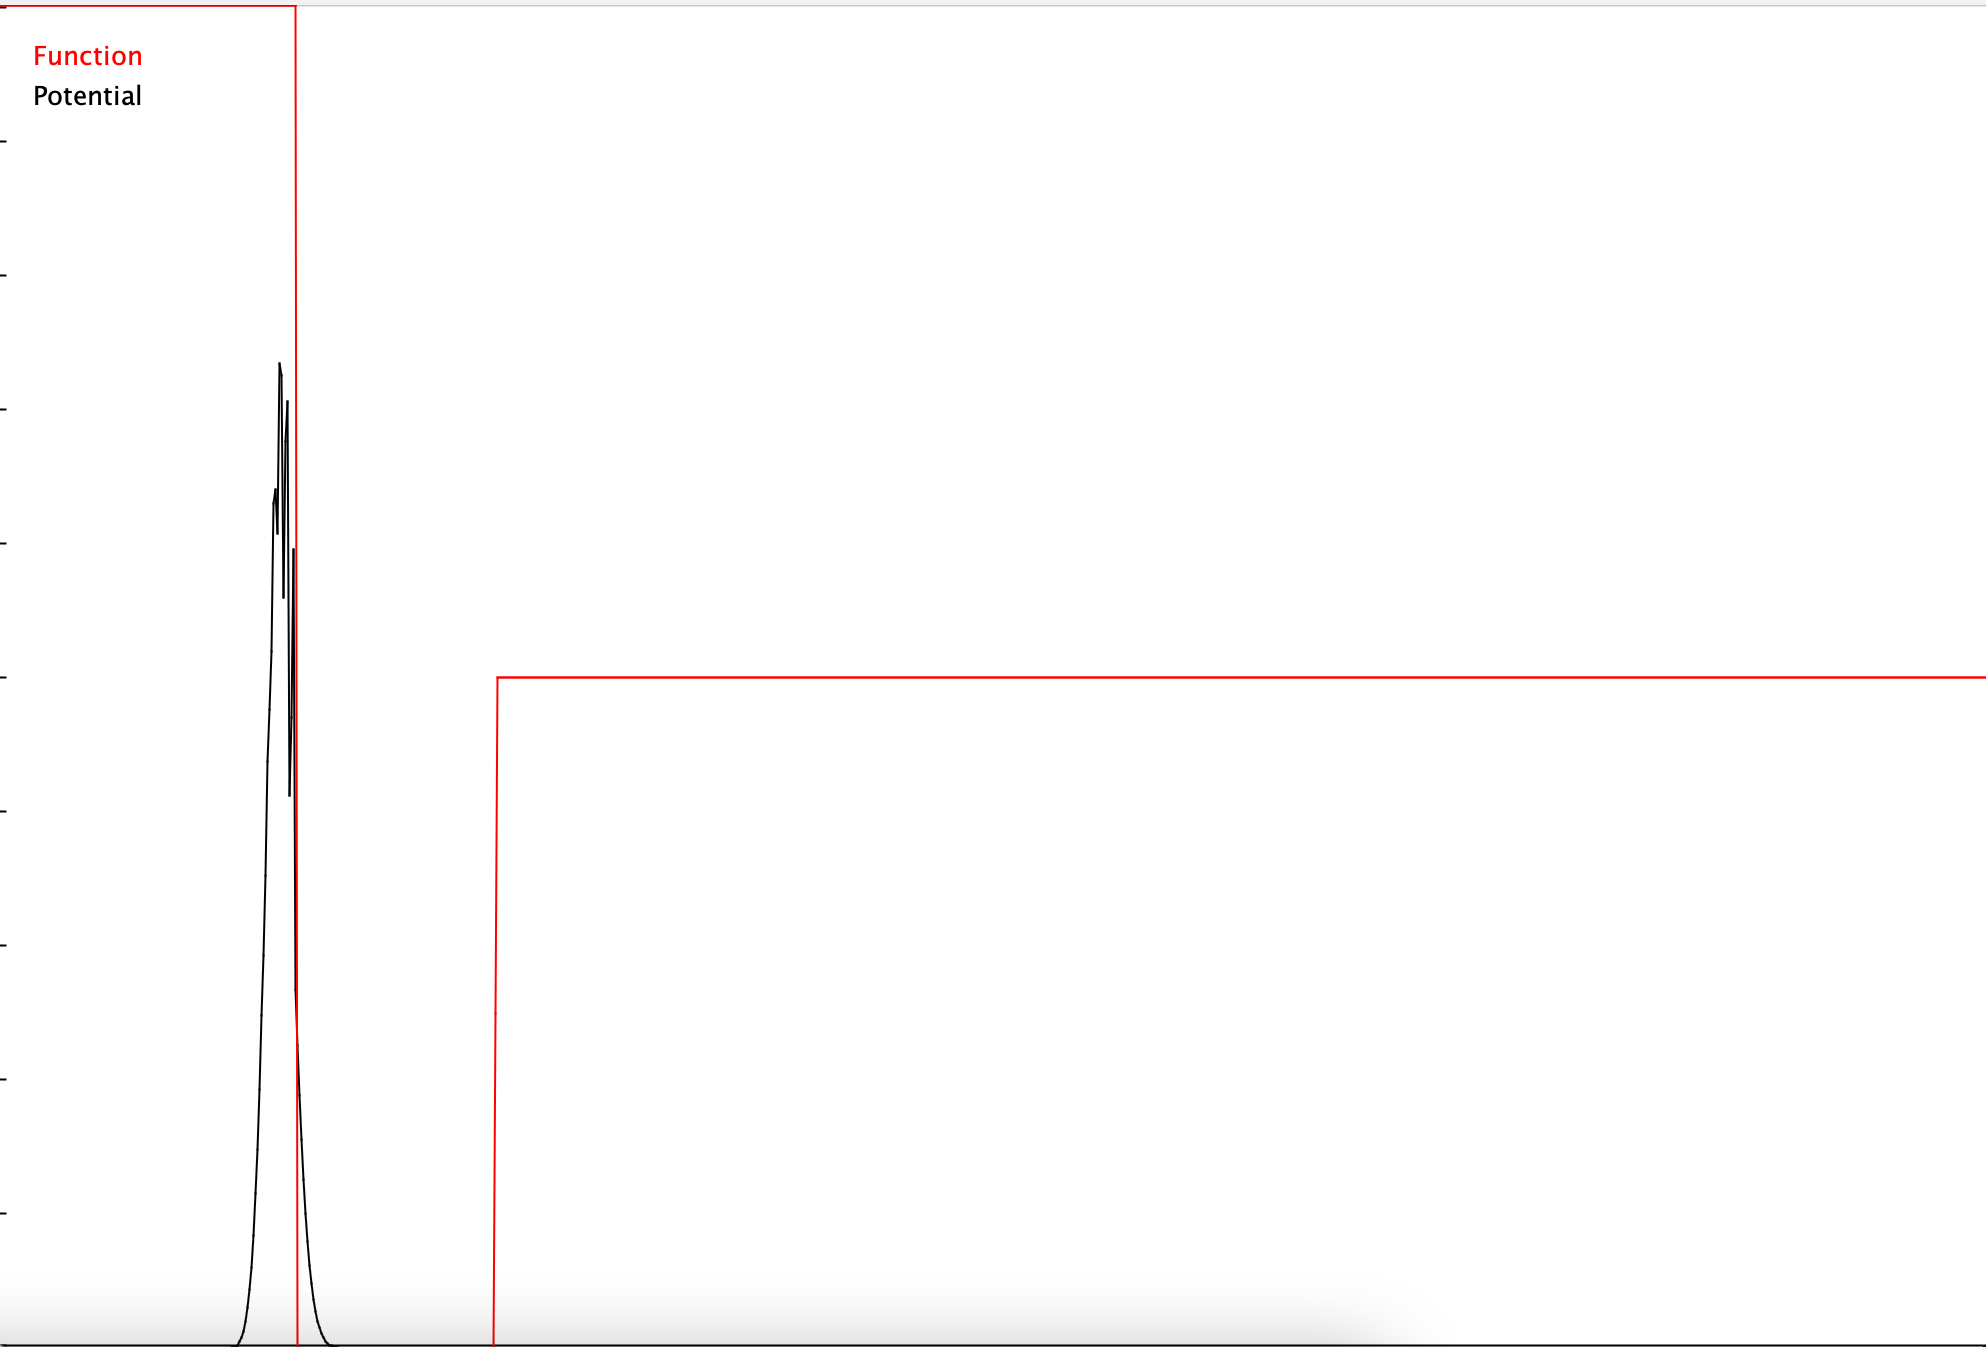
\includegraphics[width = \textwidth]{images/Screenshot 2021-03-14 at 12.50.44.png}
    \caption{Created by using the parameters: "$20*h(0-(x-0.15))+10*h(x-0.25)$", "$(1/(2*3.14159*0.005\^\ 2))\^\ (1/4)*e(0-(x-0.1)\^\ 2/(4*0.005\^\ 2))*e(200000i*x)$"}
    \label{fig:my_label}
\end{figure}
\subsection{Problems we had}
\begin{itemize}
    \item Efficiency in the inversion of $1000\times1000$ matrices $\to$ Thomas-Algorithm
    \item Visual Performance $\rightarrow$ runtime optimazition and in memory processing
\end{itemize}
\subsection{Improvements}
\begin{itemize}
    \item Bordercase behavoir (absorbing walls)
    \item Multidimensionality
\end{itemize}
\newpage

\begin{thebibliography}{9}
\bibitem{Crank-Nicolson}
Wikipedia, Crank-Nicolson method
\\\texttt{https://en.wikipedia.org/wiki/Crank-Nicolson\_method}

\bibitem{Thomas-Algorithm}
Wikipedia, Thomas Algorithm
\\\texttt{https://en.wikipedia.org/wiki/Tridiagonal\_matrix\_algorithm}

\bibitem{Script}
Prof. Dr. Alexander Lichtenstein, \textit{Computational Physics script}
\end{thebibliography}
\end{document}